%
% Zusammenfassung Communication Networks D-ITET
% ===========================================================================
% Author:			Marco Dober
% Version:			0.1
% Last changed: 	19.02.2019	
% ---------------------------------------------------------------------------

\documentclass[a4paper, fontsize=8pt, landscape, DIV=1]{scrartcl}
\usepackage{lastpage}
\usepackage{hyperref}
\usepackage{graphicx} %somehow input from general doesnt seem to work?
\usepackage{enumitem}
% Include general settings and customized commands
%
% General packages and settings
% ===========================================================================
% Author:			Silvano Cortesi (cortesis@student.ethz.ch)
% Version:			1.2
% Last changed:		03.01.2018
%
% ---------------------------------------------------------------------------




\usepackage[german,british]{babel} %choose your language \usepackage[german]{babel}
%\usepackage[T1]{fontenc}
\usepackage[utf8]{inputenc}
\usepackage{fancyhdr}
%\usepackage{lastpage}
%\usepackage{lmodern}
\usepackage{enumerate}
%\usepackage{float} % for positioning of figures
\usepackage[landscape, margin=1cm]{geometry}
\usepackage[dvipsnames]{xcolor}
\usepackage{pdfpages}


%% Math %%
\usepackage{amscd}
\usepackage{blindtext}
\usepackage{enumitem}
\usepackage{multicol}
\usepackage{parskip}
\usepackage{empheq}
\usepackage{amsmath}
\usepackage{amsfonts}
\usepackage{amssymb}
\usepackage{amsthm}
%\usepackage{adjustbox}
%\usepackage{dsfont}
%\usepackage{esint} % provides \oiint
\usepackage{mathrsfs}
%\usepackage{trfsigns}
%\numberwithin{equation}{subsection}
%\usepackage{numprint}

%% Graphics & Charts %%
\usepackage{graphicx}
%\usepackage{pdfpages}
%\usepackage{booktabs}
%\usepackage{array}
%\usepackage{paralist}
%\usepackage{framed}
%\usepackage{trfsigns}
\usepackage{tikz}
\usepackage{wrapfig}
%\usepackage[lofdepth,lotdepth]{subfig}
%\usepackage{tikz}  %Graphen zeichnen
%\usetikzlibrary{decorations.pathmorphing}
%\usetikzlibrary{arrows.meta,arrows}
%\usepackage{pgfplots}

%% General Settings %%
%\setlength{\parindent}{0px}
%\setkomafont{captionlabel}{\normalfont\bfseries}

%\pagestyle{fancy}
%\lfoot{\tiny \today}
%\rfoot{\thepage\  / \pageref{LastPage}}
%\cfoot{}
%\renewcommand{\footrulewidth}{0.4pt}

%% provides command \uline{} for underlining words
%\usepackage{ulem}

%% colour headings
%\usepackage{color}
%\definecolor{bluen}{cmyk}{1,0.5,0,0}
%\definecolor{bloodorange}{cmyk}{0,.92,1,.2}
%\addtokomafont{section}{\color{bloodorange}}
%\addtokomafont{subsection}{\color{bloodorange}}
%\addtokomafont{subsubsection}{\color{bloodorange}}
%\addtokomafont{paragraph}{\small\color{bloodorange}}
%\addtokomafont{subparagraph}{\small\color{bloodorange}}

%% Signs & Special Formating %%
%\usepackage{ulem} %normalem: \emph{Text} is italic again.
%\usepackage{multicol,multirow}
%\usepackage{tabularx}
%\usepackage{stackrel}
%\usepackage{makeidx}
%\usepackage{mparhack} % bessere margiale bei seitenumbruch

% make document compact
%\usepackage[compact]{titlesec}
%\titlespacing{\section}{0pt}{*1}{*1}
%\titlespacing{\subsection}{0pt}{*1}{*1}
%\titlespacing{\subsubsection}{0pt}{*1}{*1}

\RedeclareSectionCommand[
	%runin=false,
	%afterindent=false,
	beforeskip=3pt,
	afterskip=3pt]{section}
\RedeclareSectionCommand[
	%runin=false,
	%afterindent=false,
	beforeskip=0pt,
	afterskip=2pt]{subsection}
\RedeclareSectionCommand[
	%runin=false,
	%afterindent=false,
	beforeskip=0pt,
	afterskip=1pt]{subsubsection}

\parindent 0pt
\pagestyle{empty}
\setlength{\unitlength}{1cm}
\setlist{leftmargin = *}

%include also newer PDF
\pdfminorversion=6

% Set the color of your style
% Avaiable are: Apricot, Aquamarine, Bittersweet, Black, Blue, blue, BlueGreen, BlueViolet, BrickRed, Brown, BurntOrange, CadetBlue, CarnationPink, Cerulean, CornflowerBlue, Cyan, Dandelion, DarkOrchid, Emerald, ForestGreen, Fuchsia, Goldenrod, Gray, Green, GreenYellow, JungleGreen, Lavender, ... (more at: http://en.wikibooks.org/wiki/LaTeX/Colors)
\def\StyleColor{BrickRed}

%
% General commands
% ===========================================================================
% Author:			Silvano Cortesi (cortesis@student.ethz.ch)
% Version:			1.2
% Last changed:		03.01.2018
%
% ---------------------------------------------------------------------------

%..ROEMISCHE_ZAHLEN
	\newcommand{\Roe}[1]{\uppercase\expandafter{\romannumeral #1 }}

%..ZAHLENMENGEN
	\newcommand{\N}{\mathbb{N}}
	\newcommand{\Z}{\mathbb{Z}}
	\newcommand{\Q}{\mathbb{Q}}
	\newcommand{\R}{\mathbb{R}}
	\newcommand{\real}{\R}
	\newcommand{\C}{\mathbb{C}}
	\newcommand{\complex}{\C}
	\newcommand{\0}{\mathbb{O}}
	\newcommand{\F}{\mathbb{F}}
	\newcommand{\K}{\mathbb{K}}
    \newcommand{\angstrom}{\textup{\AA}}
    
%..PFEILE
	\renewcommand{\leadsto}{\Longrightarrow}
	\newcommand{\leftrightleadsto}{\Longleftrightarrow}

%..VEKTOREN
	\newcommand{\Ul} {\underline}
	\newcommand{\vEx} {\vec{e}_x}
	\newcommand{\vEy} {\vec{e}_y}
	\newcommand{\vEz} {\vec{e}_z}
	\newcommand{\vEq} {\vec{e_1}}
	\newcommand{\vEw} {\vec{e_2}}
	\newcommand{\vEe} {\vec{e_3}}
	\newcommand{\transpose} {^{\text{T}}}
	\newcommand{\vect}[1]{\boldsymbol{#1}}
	
%..MATRIX
    \newcommand{\MATR}[1]{ \displaystyle \left( \begin{matrix} #1 \end{matrix} \right)}
    \newcommand{\MATRABS}[1]{ \displaystyle \left| \begin{matrix} #1 \end{matrix} \right|}


%..KOMPLEXE ZAHLEN
	\renewcommand{\Re}{\text{Re}\,}
	\renewcommand{\Im}{\text{Im}\,}

%..OPERATOREN
	\DeclareMathOperator{\grad}{grad}
	\renewcommand{\div}{\text{div}\,}
    	\DeclareMathOperator{\rot}{rot}
    	\DeclareMathOperator{\divg}{div}
    	\DeclareMathOperator{\Tr}{Tr}
    	\DeclareMathOperator{\const}{const}
	\DeclareMathOperator{\imag}{i}
	\newcommand{\Lapl}{\hbox{\footnotesize{$\Delta$}}}

%..DIFFERENTIALRECHNUNG
	\newcommand{\Dx} {\,\mathrm{d}}
	\newcommand{\abl}[1] {\frac{\mathrm{d}}{\mathrm{d}#1}}
	\newcommand{\Abl}[2] {\frac{\mathrm{d}#1}{\mathrm{d}#2}}
	\newcommand{\ablq}[1] {\frac{\mathrm{d^2}}{\mathrm{d}#1^2}}
	\newcommand{\Ablq}[2] {\frac{\mathrm{d^2}#1}{\mathrm{d}#2^2}}
	\newcommand{\pabl}[1] {\frac{\partial}{\partial#1}}
	\newcommand{\pablq}[1] {\frac{\partial^2}{\partial#1^2}}
	\newcommand{\Pabl}[2] {\frac{\partial#1}{\partial#2}}
	\newcommand{\Pablq}[2] {\frac{\partial^2#1}{\partial#2^2}}

%..INTEGRALRECHNUNG
	\newcommand{\dint}{\displaystyle{\int}}
	\newcommand{\intab}{\int^b_a}
	\newcommand{\intinf}{\int_{-\infty}^\infty}
	\newcommand{\dintab}{\displaystyle{\int^b_a}}
	\newcommand{\dintpi}{\displaystyle{\int^{\pi}_{-\pi}}}
	\newcommand{\dintzpi}{\displaystyle{\int^{2\pi}_{\mbox{-}2\pi}}}
	\newcommand{\dA}{\hspace{4pt}\mathrm{d}A}
	\newcommand{\dx}{\hspace{4pt}\mathrm{d}x}
	\newcommand{\dy}{\hspace{4pt}\mathrm{d}y}
	\newcommand{\dz}{\hspace{4pt}\mathrm{d}z}
	\newcommand{\dr}{\hspace{4pt}\mathrm{d}r}
	\newcommand{\ds}{\hspace{4pt}\mathrm{d}s}
	\newcommand{\dS}{\hspace{4pt}\mathrm{d}S}
	\newcommand{\dt}{\hspace{4pt}\mathrm{d}t}
	\newcommand{\dm}{\hspace{4pt}\mathrm{d}m}
	\newcommand{\dk}{\hspace{4pt}\mathrm{d}k}
	\newcommand{\dl}{\hspace{4pt}\mathrm{d}l}
	\newcommand{\du}{\hspace{4pt}\mathrm{d}u}
	\newcommand{\dv}{\hspace{4pt}\mathrm{d}v}
	\newcommand{\dV}{\hspace{4pt}\mathrm{d}V}
	\newcommand{\dphi}{\hspace{4pt}\mathrm{d}\varphi}
	\newcommand{\domega}{\hspace{4pt}\mathrm{d}\omega}
	\newcommand{\dvarsigma}{\hspace{4pt}\mathrm{d}\varsigma}
	\newcommand{\dtau}{\hspace{4pt}\mathrm{d}\tau}
	\newcommand{\dtheta}{\hspace{4pt}\mathrm{d}\vartheta}
	\newcommand{\dmu}{\hspace{4pt}\mathrm{d}\mu}
	\newcommand{\dxi}{\hspace{4pt}\mathrm{d}\xi}
	\newcommand{\deta}{\hspace{4pt}\mathrm{d}\eta}
	\newcommand{\dvecl}{\hspace{4pt}\mathrm{d}\vec{l}}
	\newcommand{\dvecS}{\hspace{4pt}\mathrm{d}\vec{S}}

%..LIMES
    \DeclareMathOperator{\limni}{\lim\limits_{n\to\infty}}
    \DeclareMathOperator{\limxi}{\lim\limits_{x\to\infty}}
    \DeclareMathOperator{\limho}{\lim\limits_{h\to0}}
    \newcommand{\limxai}[1]{\ensuremath{\lim\limits_{x\to #1}}}

%..SUMMEN
    \DeclareMathOperator{\sumni}{\sum_{n=0}^{\infty}}
    \newcommand{\sumnia}[1]{\ensuremath{\sum_{n=#1}^{\infty}}}


%..PARTIELLE ABLEITUNG
    \DeclareMathOperator{\partf}{\dfrac{\partial f}{\partial x}}
    \newcommand{\partfo}[1]{\ensuremath{\dfrac{\partial f}{\partial #1}}}
    \newcommand{\parto}[1]{\ensuremath{\dfrac{\partial }{\partial #1}}}
    \newcommand{\partt}[2]{\ensuremath{\dfrac{\partial^2 }{\partial #1\partial #2}}}
    \newcommand{\partq}[1]{\ensuremath{\dfrac{\partial^2 }{\partial #1^2}}}


%..ENUMERATION
    \newenvironment{abc}{\begin{enumerate}[(a)]}{\end{enumerate}}
    \newenvironment{cabc}{\begin{compactenum}[(a)]}{\end{compactenum}}
    \newenvironment{romanenum}{\begin{enumerate}[i.]}{\end{enumerate}}
    \newenvironment{cromanenum}{\begin{compactenum}[i.]}{\end{compactenum}}

%..FUNCTIONS
    \DeclareMathOperator{\arsinh}{arsinh}
    \DeclareMathOperator{\arcosh}{arcosh}
    \DeclareMathOperator{\artanh}{artanh}
    \DeclareMathOperator{\arcoth}{arcoth}
    \DeclareMathOperator{\arccot}{arccot}
    \DeclareMathOperator{\Arg}{Arg}
    \DeclareMathOperator{\Log}{Log}
    \newcommand{\dis}[1]{\hspace{#1cm}}
    \newcommand{\abs}[1]{\ensuremath{\left\vert#1\right\vert}}
    \newcommand{\attention}{\raisebox{-1pt}{{\makebox[1.6em][c]{\makebox[0pt][c]{\raisebox{.13em}{\small!}}\makebox[0pt][c]{\color{red}\Large$\bigtriangleup$}}}}}
    \DeclareMathOperator{\meq}{\stackrel{!}{=}}
    
    
% section color box
\setkomafont{section}{\mysection}
\newcommand{\mysection}[1]{%
    \Large\sffamily\bfseries%
    \setlength{\fboxsep}{0cm}%already boxed
    \colorbox{\StyleColor!40}{%
        \begin{minipage}{\linewidth}%
            \vspace*{3pt}%Space before
            #1
            \vspace*{1pt}%Space after
        \end{minipage}%
    }}

%subsection color box
\setkomafont{subsection}{\mysubsection}
\newcommand{\mysubsection}[1]{%
    \normalsize \sffamily\bfseries%
    \setlength{\fboxsep}{0cm}%already boxed
    \colorbox{\StyleColor!20}{%
        \begin{minipage}{\linewidth}%
            \vspace*{2pt}%Space before
             #1
            \vspace*{-1pt}%Space after
        \end{minipage}%
    }}

%subsubsection color box
\setkomafont{subsubsection}{\mysubsubsection}
\newcommand{\mysubsubsection}[1]{%
	\normalsize \sffamily\bfseries%
	\setlength{\fboxsep}{0cm}%already boxed
	\colorbox{\StyleColor!10}{%
		\begin{minipage}{\linewidth}%
			\vspace*{2pt}%Space before
			#1
			\vspace*{-1pt}%Space after
		\end{minipage}%
	}}

% highlighter
\newcommand{\hilight}[1]{\colorbox{\StyleColor}{#1}}
\newcommand{\highlighty}[1]{%
  \setlength{\fboxsep}{0pt}\colorbox{yellow!100}{\ensuremath{#1}}}

\newcommand{\highlightg}[1]{%
  \setlength{\fboxsep}{0pt}\colorbox{green!100}{\ensuremath{#1}}}

\newcommand{\highlightbg}[1]{%
   \colorbox{green!100}{$\displaystyle #1$}}  

% equation box        
\newcommand{\eqbox}[1]{\setlength{\fboxrule}{1mm}\fcolorbox{\StyleColor}{white}{\hspace{0.5em}$\displaystyle#1$\hspace{0.5em}}}

%center equationbox
\newcommand{\ceqbox}[1]{\vspace*{4pt} \begin{center}\eqbox{#1}\end{center}\vspace*{4pt}}

%change page style for header
\pagestyle{fancy}
\footskip 20pt
\rhead{Marco Dober}
\lhead{Introduction to Machine Learning}
\chead{\thepage}
\cfoot{}
\headheight 17pt \headsep 10pt
\title{Introduction to Machine Learning}
\author{Marco Dober}
\date{\today}


\begin{document}
	\setcounter{secnumdepth}{3} %no enumeration of sections
	\begin{multicols*}{4}
		%
%		\section*{Disclaimer}
%			This should be a summary of the Communication Networks course. The goal is to update it weekly with the currently taught material.  	
%			\pagebreak

		\maketitle 
		\thispagestyle{fancy}
		
		\section{Introduction}
		There exists two basic forms of learning:
		\begin{itemize}[noitemsep]
			\item \textbf{Supervised learning}\\
			You have data with x- and y-labels $\rightarrow$ try to fit model $\rightarrow$ predict with found model new cases. Examples of supervised learning:
			\begin{itemize}
				\item Classification
				\item Regression
				\item Structured prediction, ...
			\end{itemize}
			Model selection is very important and a trade off between complexity vs. goodness of fit. Ideal models are statistically and computationally efficient. 
			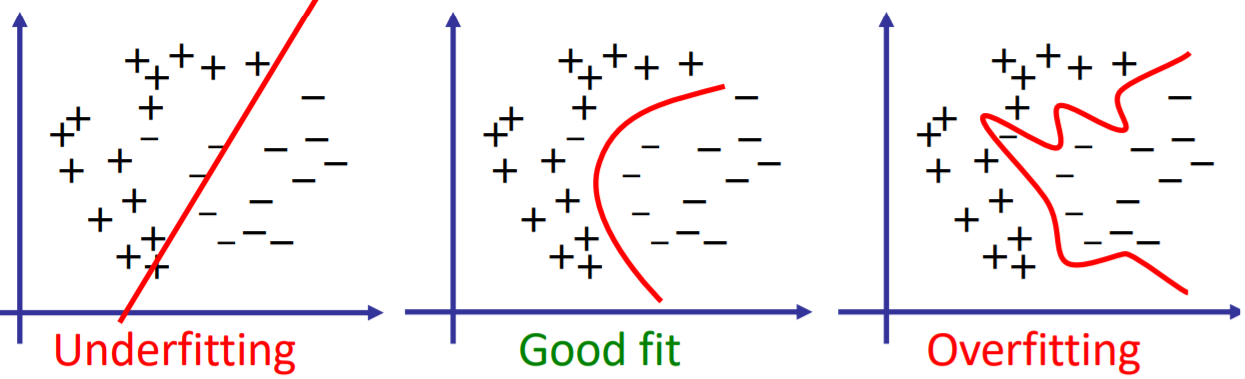
\includegraphics[width=\columnwidth]{images/Introduction/model_selection.png}
			\item \textbf{Unsupervised learning}\\
			"Learning without labels" (no y-label on data). Examples:
			\begin{itemize}[noitemsep]
				\item Clustering (e.g., unsupervised classification)
				\item Dimension reduction (e.g., unsupervised regression)
				\item Generative modeling
			\end{itemize}
			Common goals: 
			\begin{itemize}
				\item Compact representation / compression of data sets
				\item Identification of latent variables
			\end{itemize}
		\end{itemize}
		Example of unsupervised learning, Clustering: Input data with no labels and assign data to clusters
		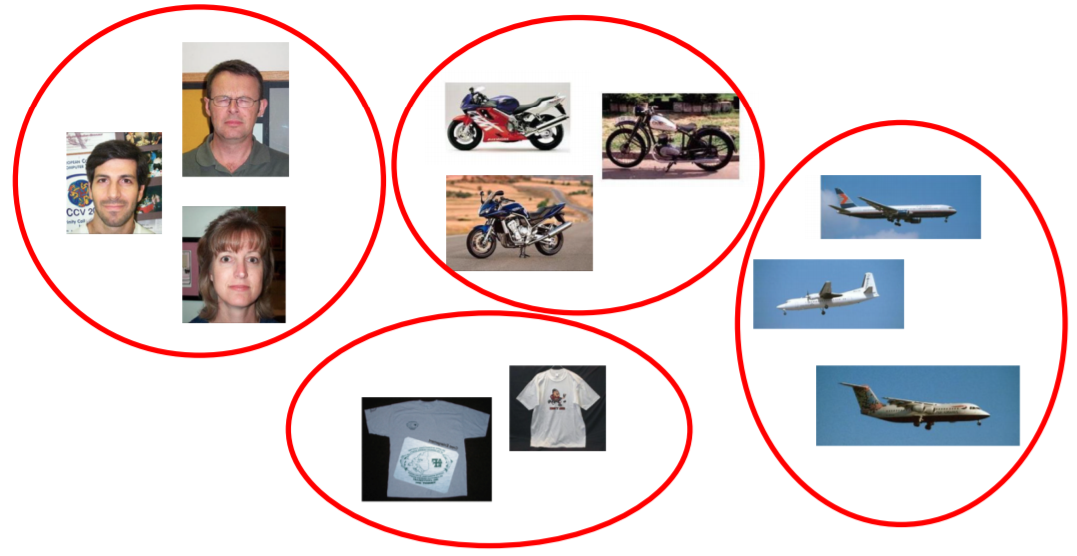
\includegraphics[width=0.85\columnwidth]{images/Introduction/clustering.png}\\
		Other models of learning: semi-supervised, transfer, active, online, reinforcement, ... .\\
		The key challenge in ML is: \\
		$\bullet$ Trading goodness of fit and model complexity\\
		$\bullet$ Also the \textbf{representation of data} is of key importance. 
		
		\section{Regression}
		Is an instance of supervised learning.\\
		\textbf{Goal:} Predict real valued labels.\\
		Important choices in regression:
		\vspace{-0.1cm}
		\begin{itemize}[noitemsep,nolistsep]
			\item What \textbf{types of functions} should we consider?
			\item How should we measure \textbf{goodness of fit}?
		\end{itemize}
	
		\subsection{Linear Regression}
		$y\approx f(x)$, $f$ is linear (affine) in $x$
		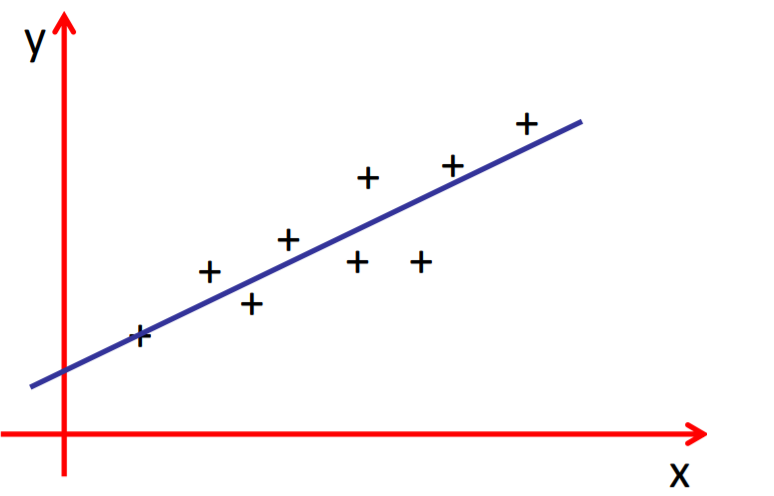
\includegraphics[width=\columnwidth]{images/Regression/linear_regression.png}
		\begin{itemize}[noitemsep]
			\item 1-d: $f(x)=ax+b$, (line)
			\item 2-d: $f(x)=ax_1+bx_2+c$, (area)
			\item d-d: $f(x)=w_1x_1+\dots+w_dx_d+w_0=\\\sum_{i=1}^{d}w_ix_i+w_0=w^Tx+w_0$\\
			$w=[w_1,\dots,w_d]^T$, $x=[x_1,\dots,x_d]^T$
		\end{itemize}
		Homogeneous representation (no offset):\\
		$w^Tx+w_0=\tilde{w}^T\tilde{x}$\\
		$\tilde{w}=[w_1,\dots,w_d,w_0]^T$, $\tilde{x}=[x_1,\dots,x_d,1]^T$\\
		
		\subsubsection{Quantifying goodness of fit}
		Calculate \textbf{residuals}, difference from fitet-point and data-point. Different ways to compute loss function (abs-value, square, ...), see below. Most famous is the \textbf{least-square optimization}: \\
		$r_i=y_i-f(x_i)=y_i-w^Tx_i$\\
		Cost $\hat{R}(w)=\sum_{i=1}^{n}r_i^2=\sum_{i=1}^{n}(y_i-w^Tx_i)^2$\\
		How do we find the optimal weight vector $w^*$?
		\begin{equation*}
			w^*=\arg\min\limits_w\sum_{i=1}^{n}(y_i-w^Tx_i)^2 
		\end{equation*}
		\columnbreak
		
		$\bullet$ \textbf{Closed form}\\
		The problem from above can be solved in closed form!
		\begin{equation*}
			w^*=(X^TX)^{-1}X^Ty
		\end{equation*}
		$X=\begin{pmatrix} x_{1,1} & \dots & x_1,d \\ \dots & \dots & \dots \\ x_{n,1} & \dots & x_{n,d} \end{pmatrix}$, $y=\begin{pmatrix} y_1 \\ \dots \\ y_n \end{pmatrix}$\\
		\vspace{0.1cm}
		
		$\bullet$ \textbf{Optimization}\\
		The objective function is \textbf{convex}. In convex functions local minimum = global minimum!
		\vspace{0.1cm}
		
		\textbf{Gradient descent}:\\
		- Start at arbitrary $w_0 \in \R^d$\\
		- For $t=1,2,...$ do
		\begin{equation*}
			w_{t+1}=w_t-\eta_t\nabla\hat{R}(w_t)
		\end{equation*}
		If I descend along the gradient I will for sure find a minimum (step size / learning rate $\eta_t$ sufficiently small). For convex objectives it finds an optimum. For the squared loss, \textbf{constant step size 0.5 converges linearly}!\\
		$\nabla\hat{R}(w)=\dots=-2\sum_{i}^{n}r_ix_i^T$, (in all dimensions)
		\vspace{0.1cm}
		
		\textbf{Adaptive step size}\\
		- step size too big: oscillation, divergence\\
		- step size too small: long computation\\
		Different ways to update step size adaptively: 
		\begin{enumerate}[noitemsep]
			\item Line search (optimizing step size every step)\\
			$g_t=\nabla\hat{R}(w_t)$\\
			$\eta_t = \arg \min\limits_{\eta\in(0,\inf)}\hat{R}(w_t-\eta g_t)$
			\item Bold driver heuristic
			\begin{itemize}
				\item If function decreases, increase step size:\\
				$\hat{R}(w_t-\eta_t g_t)<\hat{R}(w_t)\Rightarrow \eta_{t+1}=\eta_t\cdot c_{acc.}$ 
				\item If function increases, decrease step size:\\
				$\hat{R}(w_t-\eta_t g_t)>\hat{R}(w_t)\Rightarrow \eta_{t+1}=\eta_t\cdot c_{dec.}$\\
				$c_{acc.}>1$ \& $c_{dec.}<1$
			\end{itemize}
		\end{enumerate}
		\textbf{Gradient descent vs. closed form} (many times gradient descent (optimization) is better than closed form):
		\vspace{-0.2cm} 
		\begin{itemize}[noitemsep]
			\item computational complexity:\\
			 closed form can get very ugly (shit-ton of calculations)
			\item May not need an optimal solution:\\
			Uncertainty in data, so it makes no sense to find the optimal solution, I can stop earlier with optimization.
			\item Many problems don't admit closed form solution
		\end{itemize}
		\columnbreak
		
		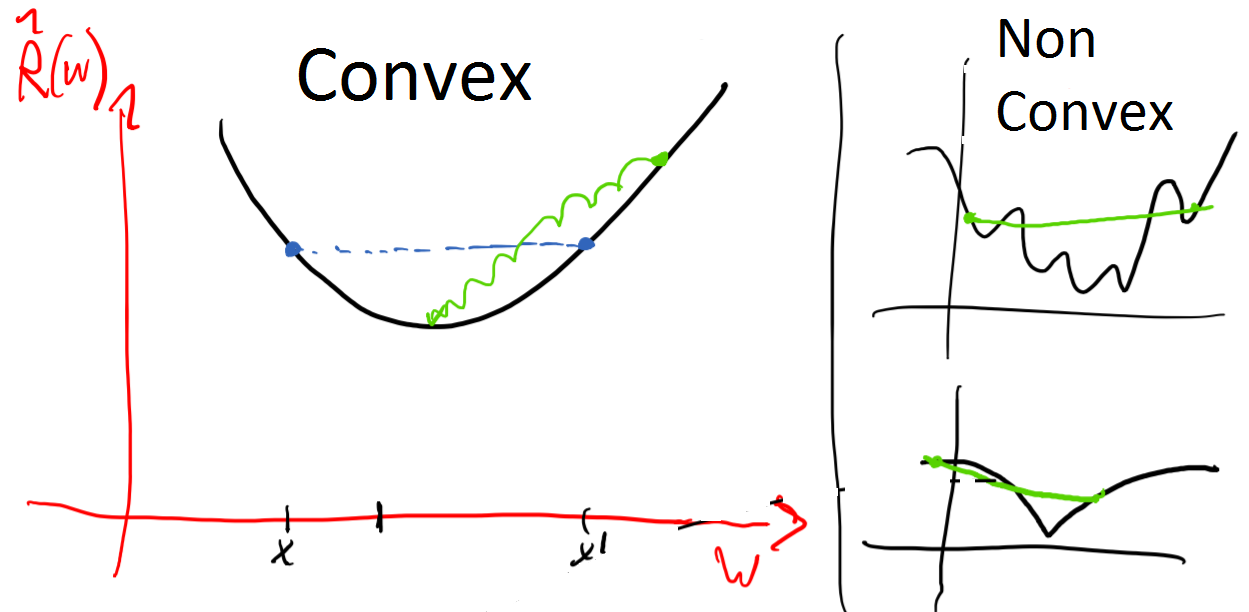
\includegraphics[width=\columnwidth]{images/Regression/convex_nonconvex.png}
		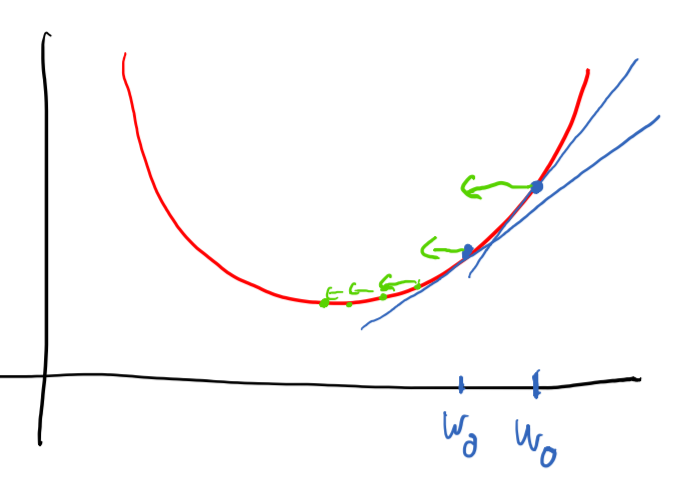
\includegraphics[width=\columnwidth]{images/Regression/gradient_descent.png}
		\subsubsection{Other loss functions}
		so far we used squared error to measure goodness of fit, but there are many other possibilities. 
		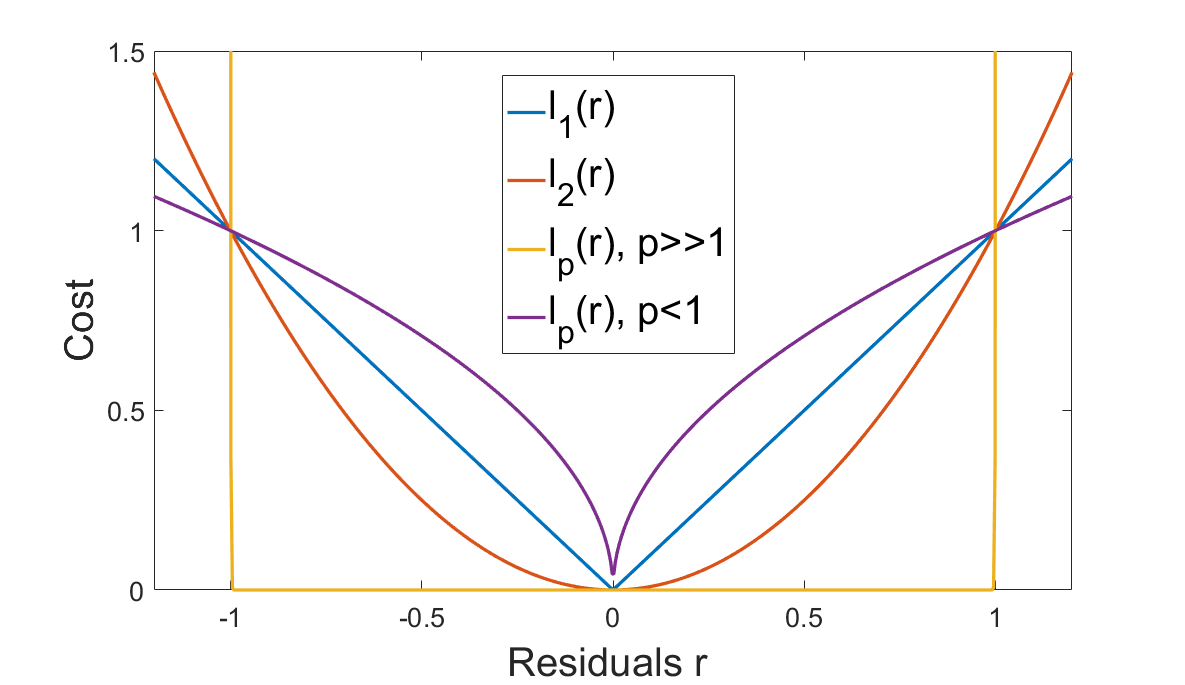
\includegraphics[width=\columnwidth]{images/Regression/loss_functions.png}
	 	$l_p(r)=\abs{r}^p=\abs{y_i-w^Tx_i}^p$, with the parameter $p$ you can vary your optimization. 
	 	\begin{itemize}[noitemsep]
	 		\item $p=1$: weight all $r$ the same, less sensible to outliers 
	 		\item $p=2$: closed form sol., most common
	 		\item $p>>1$: make tolerance band of allowed errors
	 		\item $p<<1$: almost no weight to outliers
	 	\end{itemize}
		$\hat{R}(w)=\sum_{i=1}^{n}l_p(y_i-w^Tx_i)$
		\newpage 
		
		\subsection{Fitting nonlinear functions}
		We can fit nonlinear functions via linear regression using nonlinear features of our data (basis functions). With a nonlinear transformation we transform data to be able to fit linearly.\\
		.... 
	\end{multicols*}
	\setcounter{secnumdepth}{3}
\end{document}

